\documentclass{article}
\usepackage{tikz}
\usepackage{tikz-3dplot}
\usepackage{amsmath}

\usepackage[dvipsnames]{xcolor}


\begin{document}

\tdplotsetmaincoords{70}{120} % Define viewing angles (adjust as needed)

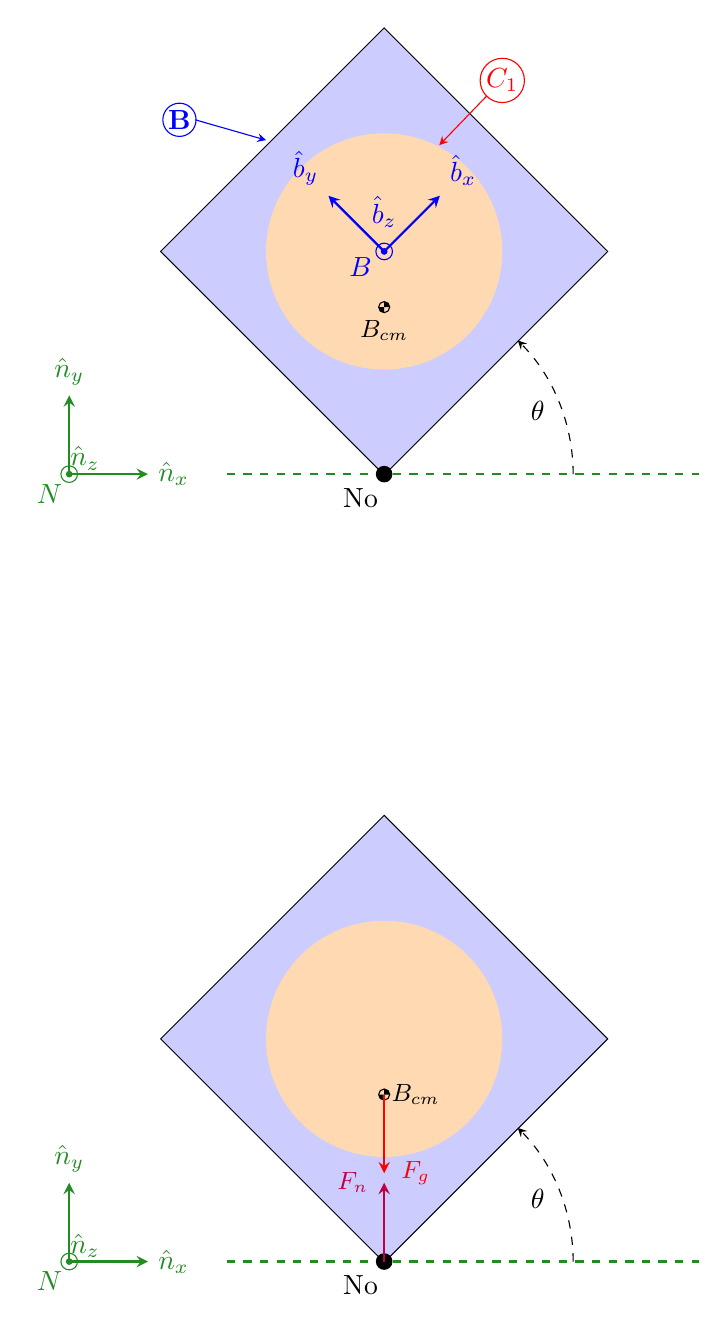
\begin{tikzpicture}[>=stealth] % >=stealth ensures nice arrowheads

    % 1. Define the length of the axes
    \def\axlen{1}
    % 2. Define the radius of the rotation arc
    \def\arcrad{0.4}

    % --- Draw the X and Y axes (flat on the page) ---
    % set the color of this frame to be ForestGreen
    
    % X-Axis
    \draw[->, thick, ForestGreen] (0, 0) -- (\axlen, 0) node[right] {$\hat{n}_x$};
    % Y-Axis
    \draw[->, thick, ForestGreen] (0, 0) -- (0, \axlen) node[above] {$\hat{n}_y$};

    % Label the ref frame as N to the bottom left of the origin
    \node[ForestGreen] at (-0.25, -0.25) {$N$};

    % --- Draw the Z-axis Representation ---

    % % 1. Draw the rotation arc (from X axis (0 deg) to Y axis (90 deg))
    % % The use of the segment 0-90 defines the positive rotation direction.
    % \draw[->, thin, dashed] (\arcrad, 0) arc (0:90:\arcrad);

    % Draw a square to represent the cube face cube should have left point at (2,0) and be 4x4 should be at 45 degree angle
    % The square represents the face of the cube in the reference frame. (write in terms of angle 45 degrees double the side length)
    \draw[thick] (4,0) -- (4+4*0.707, 4*0.707) -- (4, 8*0.707) -- (4-4*0.707, 4*0.707) -- cycle;
    % fill square with light blue
    \fill[blue!20] (4,0) -- (4+4*0.707, 4*0.707) -- (4, 8*0.707) -- (4-4*0.707, 4*0.707) -- cycle;



    % Draw a dashed arc to label the angle theta between the x axis and the second line on the square
    \draw[->, thin, dashed] (6+1*\arcrad, 0) arc (0:45:6*\arcrad);
    % Label the angle theta
    \node[black] at (5.75+0.5*\arcrad, 2*\arcrad) {$\theta$};
    % Draw a dashed line from the origin to the point (4,0)
    \draw[thick, dashed, ForestGreen] (2,0) -- (8,0);
    % Label bottom point as No
    \node at (4-0.3, -0.3) {No};
    % point a point there too at that corner
    \fill (4,0) circle (3pt);
    % 2. (Optional but common) Draw the Z-axis symbol
    % A circle with a dot in the center means the vector is pointing OUT of the page (towards the viewer).
    \draw[fill=black, ForestGreen] (0, 0) circle (1pt);
    \draw[thin, ForestGreen] (0, 0) circle (3pt);

    % make a circle that is in the center of the square that is filled with a light organge color
    \fill[orange!30] (4, 4*0.707) circle (1.5);

    % make center of gravity symbol at the center of the square that is like circle with two quarters filled in make it 4pt diameter fill to center
    \draw[thin] (4, 3*0.707) circle (2pt);
    \fill[black] (4, 3*0.707) -- ++(2pt,0) arc (0:90:2pt) -- cycle;
    \fill[black] (4, 3*0.707) -- ++(-2pt,0) arc (180:270:2pt) -- cycle;
    % label as B sub cm in small font
    \node at (4, 3*0.707-0.3) {\small $B_{cm}$};

    % In blue make a circle with a capital B in the center and an arrow point to the square
    % circle
    \draw[blue] (1.4,4.5) circle (6pt);
    % arc arrow from circle to square center of side (2, 6*0.707)
    \node[blue] at (1.4,4.5) {\textbf{B}};
    % arrow
    \draw[->, blue] (1.6,4.5) -- (2.5, 6*0.707);

    % in blue at the cetner of the circle make another reference frame that is b and is aligned with the cube
    % draw the x and y axes of the b frame
    % X-Axis (center of square to
    \draw[->, thick, blue] (4, 4*0.707) -- (4+1*0.707, 4*0.707 + 1*0.707) node[above right] {\textbf{$\hat{b}_x$}};
    % Y-Axis
    \draw[->, thick, blue] (4, 4*0.707) -- (4-1*0.707, 4*0.707 + 1*0.707) node[above left] {\textbf{$\hat{b}_y$}};
    % Label the ref frame as B to the bottom left of the origin
    \node[blue] at (4-0.3, 4*0.707-0.2) {$B$};
    % Draw the Z-axis symbol for the B frame
    % A circle with a dot in the center means the vector is pointing OUT of the page (towards the viewer).
    \draw[fill=black, blue] (4, 4*0.707) circle (1pt);
    \draw[thin, blue] (4, 4*0.707) circle (3pt);
    % Label the Z-axis near the origin of the B frame
    \node[blue] at (4, 4*0.707+0.5) {$\hat{b}_z$};

    % Label the Z-axis near the origin % needs to be n with hat sub z
    \node[ForestGreen] at (0.5*\arcrad, 0.5*\arcrad) {$\hat{n}_z$};
    % Label the origin (optional)
    % \fill (0,0) circle (1.5pt) node[below left] {$O$};

    % label the orange circle as body C it should be a C in a red cirlce with an arrow pointing to the circle
    \draw[red] (5.5,5) circle (8pt);
    \node[red] at (5.5,5) {\textbf{$C_{1}$}};
    \draw[->, red] (5.5-0.2,5-0.2) -- (4.7, 4*0.707+1.35);

    % % on top of the b reference frame make a new reference frame c that is aligned with n 
    % % X-Axis
    % \draw[->, thick, red] (4, 4*0.707) -- (4+1, 4*0.707) node[right] {\textbf{$\hat{c}_x$}};
    % % Y-Axis
    % \draw[->, thick, red] (4, 4*0.707) -- (4, 4*0.707 + 1) node[above left] {\textbf{$\hat{c}_y$}};
    % % Label the ref frame as C to the bottom left of the origin
    % \node[red] at (40.3, 4*0.707-0.2) {$C$};
    % % Draw the Z-axis symbol for the C frame


    % -----------------------------------------------------------------

    % Below this drawing I want another cube at a 45 degree angle with the same n reference frame and circle
    % square should be at (4,-10)
    \draw[thick] (4,-10) -- (4+4*0.707, -10+4*0.707) -- (4, -10+8*0.707) -- (4-4*0.707, -10+4*0.707) -- cycle;
    % fill square with light blue
    \fill[blue!20] (4,-10) -- (4+4*0.707, -10+4*0.707) -- (4, -10+8*0.707) -- (4-4*0.707, -10+4*0.707) -- cycle;
    % Draw a dashed arc to label the angle theta between the x axis and the second line on the square
    \draw[->, thin, dashed] (6+1*\arcrad, -10) arc (0:45:6*\arcrad);
    % Label the angle theta
    \node[black] at (5.75+0.5*\arcrad, -10+2*\arcrad) {$\theta$};
    % Draw a dashed line from the origin to the point (4,0)
    \draw[thick, dashed, ForestGreen] (2,-10) -- (8,-10);
    % Label bottom point as No
    \node at (4-0.3, -10-0.3) {No};
    % point a point there too at that corner
    \fill (4,-10) circle (3pt);
    % make a circle that is in the center of the square that is filled with a light
    \fill[orange!30] (4, -10+4*0.707) circle (1.5);
    % make center of gravity symbol at the center of the square that is like circle with two quarters filled in make it 4pt diameter fill to center
    \draw[thin] (4, -10+3*0.707) circle (2pt);
    \fill[black] (4, -10+3*0.707) -- ++(2pt,0) arc (0:90:2pt) -- cycle;
    \fill[black] (4, -10+3*0.707) -- ++(-2pt,0) arc (180:270:2pt) -- cycle;
    % label as B sub cm in small font
    \node at (4 + 0.4, -10+3*0.707) {\small $B_{cm}$};

    % add n reference frame again
    % X-Axis
    \draw[->, thick, ForestGreen] (0, -10) -- (\axlen, -10) node[right] {$\hat{n}_x$};
    % Y-Axis
    \draw[->, thick, ForestGreen] (0, -10) -- (0, -10+\axlen) node[above] {$\hat{n}_y$};
    % Label the ref frame as N to the bottom left of the origin
    \node[ForestGreen] at (-0.25, -10.25) {$N$};
    % Draw the Z-axis symbol for the N frame
    % A circle with a dot in the center means the vector is pointing OUT of the page (towards the viewer).
    \draw[fill=black, ForestGreen] (0, -10) circle (1pt);
    \draw[thin, ForestGreen] (0, -10) circle (3pt);
    % Label the Z-axis near the origin of the N frame
    \node[ForestGreen] at (0.5*\arcrad, -10+0.5*\arcrad) {$\hat{n}_z$}; 

    % add a Fg vector in red from the center of gravity straight down
    \draw[->, thick, red] (4, -10+3*0.707) -- (4, -10+3*0.707-1) node[below] {};
    % add a label in red near the Fg vector that says Fg
    \node[red] at (4 + 0.4, -10+3*0.707-1) {\small $F_g$};

    % add normal force vector in purple from the center of gravity straight up
    \draw[->, thick, purple] (4, -10) -- (4, -10+1) node[above] {};
    % add a label in purple near the normal force vector that says Fn
    \node[purple] at (4 - 0.4, -10+1) {\small $F_n$};

    % start a new page
    \pagebreak
    


\end{tikzpicture}

\end{document}